Наряду c теоретическими математическими моделями при
функциональном проектировании технических систем широко применяются
экспериментальные факторные математические модели.

Теоретические модели имеют то преимущество, что они непосредственно
описывают физические свойства технической системы. Коэффициенты
уравнений теоретических моделей представляют собой параметры элементов
технической системы (внутренние параметры системы) или некоторые
комбинации этих параметров, а зависимые переменные – фазовые координаты
системы. Они позволяют осуществлять имитационное моделирование процессов
функционирования технической системы во времени, детально изучать
изменение фазовых координат в зависимости от внешних воздействий
(возмущающих и управляющих), анализировать устойчивость системы, качество
переходных процессов, эффективность функционирования в условиях
случайных внешних воздействий, близких к реальным, то есть оценивать ее
функциональную работоспособность и выполнение технических требований к
системе~\cite{modeling:2004}.

Но функциональные теоретические модели сложных технических
объектов представляют собой системы нелинейных дифференциальных
уравнений высокого порядка Целью функционального проектирования является
выбор структуры на основе некоторого множества вариантов и определение
оптимальных параметров технического объекта. Процедуры выбора структуры
и оптимизационные алгоритмы требуют выполнения множества итераций,
количество которых может достигать чисел второго и третьего порядков,
причем, на каждой итерации решается исходная система дифференциальных уравнений. Поэтому решение одной проектной задачи характеризуется
огромными затратами машинного времени. Этим объясняется медленное
внедрение методов функционального проектирования в конструкторских
организациях. Вместе с тем без выполнения работ по функциональному
проектированию невозможно обеспечить высокий технический уровень и
конкурентоспособность создаваемых сложных технических объектов. Затраты
машинного времени можно значительно сократить, если на этапе оптимизации
параметров использовать экспериментальную факторную математическую
модель. Экспериментальные факторные модели, B отличие от теоретических, не
используют физических законов, описывающих происходящие в объектах
процессы, а представляют собой некоторые формальные зависимости выходных
параметров от внутренних и внешних параметров объектов проектирования.

Экспериментальная факторная модель может быть построена на основе
проведения экспериментов непосредственно на самом техническом объекте
(физические эксперименты), либо вычислительных экспериментов на ЭВМ с
теоретической моделью. При создании новых технических объектов физический
эксперимент проводится на прототипах или аналогах, а иногда на макетных
образцах. Однако физические эксперименты требуют огромных затрат
материальных и временных ресурсов, поэтому их выполняют обычно в тех
случаях, когда возникает необходимость поиска путей совершенствования
существующих технических систем, когда сложность этих систем и условий их
функционирования не позволяет надеяться на требуемую точность их
математического описания теоретическими методами. При функциональном
проектировании факторные модели наиболее часто получают на основе
вычислительных экспериментов на ЭВМ с теоретической моделью. 

Схема объекта
моделирования (процесс $pp \rightarrow W^+W^- + X$) представлена на рисунке~\ref{fig:schema-model}.

\begin{figure}[!h]
	\centering
	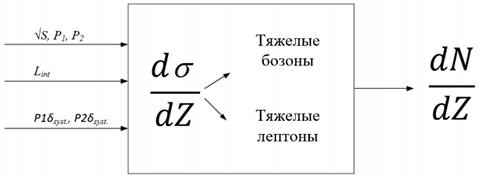
\includegraphics[width=\textwidth]{figures/imitation-schema.png}
	\caption{Схема объекта исследования при построении экспериментальной
		факторной модели}
	\label{fig:schema-model}
\end{figure}

Входными переменными являются $\sqrt{s}$, ${P}_{1}$, ${P}_{2}$, ${L}_{int}$, $P\textit{1}{\delta}_{syst}$, $P\textit{2}{\delta}_{syst}$. 

При построении экспериментальной факторной модели объект
моделирования (проектируемая техническая система) представляется в виде
«черного ящика», на вход которого подаются некоторые переменные, a на
выходе можно наблюдать и регистрировать переменные. 

Они являются внутренними и внешними параметрами объекта проектирования,
подлежащие оптимизации, а выходными переменными <<черного ящика>>
являются выходные параметры объекта, характеризующие его эффективность и
качество процессов функционирования, выбираемые в качестве критериев
оптимальности. В процессе проведения эксперимента изменение входных
переменных приводит к изменениям выходных переменных. Для построения
факторной модели были зарегистрированы эти изменения и осуществлена
необходимая статистическая обработка для определения параметров модели.